\section{Lorentz Model for Permittivity}
Recall that in the dynamical case when materials are subject to time-varying electric/magnetic fields, our work in the static regime no longer applies - in particular going to the dynamic case the permittivity picks up a frequency dependence $\e(\omega)$. We assume $\avg{\rho_f} = \avg{\v{J}_f} = 0$ and $\mu(\omega) = \mu_0$.

Individual charges in the material satisfy:
\begin{equation}
    m\ddot{\v{x}} + m\gamma\dot{\v{x}} + m\omega_0^2(\v{x} - \v{x}_0) = -e\v{E}
\end{equation}
We consider a couple cases:
\begin{itemize}
    \item Non-conducting ($\omega_0^2 > 0$)
    \item Plasma ($\omega_0 = 0, \gamma > 0$)
    \item Conductors ($\omega_0^2 > 0$ for the valence electrons, other electrons are bound)
\end{itemize}

In this setup, we discuss how each of the quantities we introduced last time behave.

\subsection{Solving for the Lorentz permittivity}
We assume a sinusoidally varying electric field:
\begin{equation}
    \v{E} = e^{-i\omega t}\hat{\v{E}}(\omega)
\end{equation}
Working in frequency space:
\begin{equation}\label{eq:freqspace}
    m(-\omega^2 - i\omega \gamma + \omega_0^2)\hat{\v{x}}(\omega) = -e\avg{\hat{\v{E}}(\omega)}
\end{equation}
Studying the dipole moment:
\begin{equation}
    \v{p}(t) = -e\v{x}(t)
\end{equation}
The fourier transform of which, using Eq. \eqref{eq:freqspace} equals:
\begin{equation}
    \hat{\v{p}}(\omega) = \frac{e^2/m}{\omega_0^2 - \omega^2 - i\omega\gamma}\avg{\hat{\v{E}}(\omega)}
\end{equation} 
The $\v{x}, \v{p}$ we discuss are for a particular particle, so we can sum over different particles. If we then combine this with:
\begin{equation}
    \avg{\hat{\v{p}}(\omega)} = \e_0\chi(\omega)\avg{\hat{\v{E}}(\omega)}
\end{equation}
we obtain:
\begin{equation}
    \chi(\omega) = \frac{e^2}{e_0m}\sum_j \frac{N_j}{\omega_j^2 - \omega^2 - i\omega\gamma_j}
\end{equation}
where $N_j$ is the number of electrons in state $j$.

Note that $\chi(\omega)$ can be analyticcally continued to $\omega$ in the upper half plane, which yields the Kramers-Kronig model we discussed.

the permittivity is obtained as:
\begin{equation}
    \frac{\e(\omega)}{\e_0} = 1 + \chi(\omega) = 1 + \sum_j \frac{N_j}{\omega_j^2 - \omega^2 - i\omega\gamma_j}
\end{equation}

for the next half hour, we discuss the implication of the above formula for physics.

\subsection{Lorentz conductivity}
The current in matter is:
\begin{equation}
    \avg{\v{J}} = \avg{\v{J}_f} = \nabla \times \avg{\v{M}} + \dpd{}{t}\avg{\v{p}}
\end{equation}
We assume no free currents, and $\avg{\v{M}} = 0$ since we take $\mu(\omega) = \mu_0$. So:
\begin{equation}
    \avg{\v{J}(\v{x}, t)} = \dpd{}{t}\avg{\v{p}(\v{x}, t)}
\end{equation}
or in frequency space:
\begin{equation}
    \avg{\hat{\v{J}}(\omega)} = -i\omega \e_0 \chi(\omega)\avg{\hat{\v{E}}(\omega)} = \sigma(\omega)\avg{\hat{\v{E}}(\omega)} 
\end{equation}
with $\sigma(\omega)$ the \emph{conductivity}. Thus:
\begin{equation}
    \sigma(\omega) = - i\omega\frac{e^2}{m}\sum_j \frac{N_j}{\omega_j^2 - \omega^2 - i\omega \gamma_j}
\end{equation}
which is $V=IR$ on steroids. 

\subsection{Different Cases}
Note that this is in no way an exact model, but we can explore its implications given its simplicity and the fact that it is analytically solvable.

\begin{itemize}
    \item \emph{Non-conducting medium.} In this case $\omega_j^2 > 0$ and $\gamma_j \ll \omega_j$, i.e. the oscillators are heavily underdamped. For most $\omega$s, it is the case that $\sigma(\omega)$ is approximately real, and as $\omega \to \omega_j$ the imaginary part of $\sigma(\omega)$ grows, leading to absorption.

    Let's study the real part of the susceptibility:
    \begin{equation}
        \text{Re}[\chi(\omega)] \sim \text{Re}\frac{1}{\omega_j^2 - \omega^2 - i\omega\gamma} = \frac{\omega_j^2 - \omega^2}{(\omega_j^2 - \omega^2)^2 + \omega^2\omega_j^2}
    \end{equation}
    for $\omega < \omega_j$, this is positive and for $\omega > \omega_j$, this is negative.

    \begin{center}
        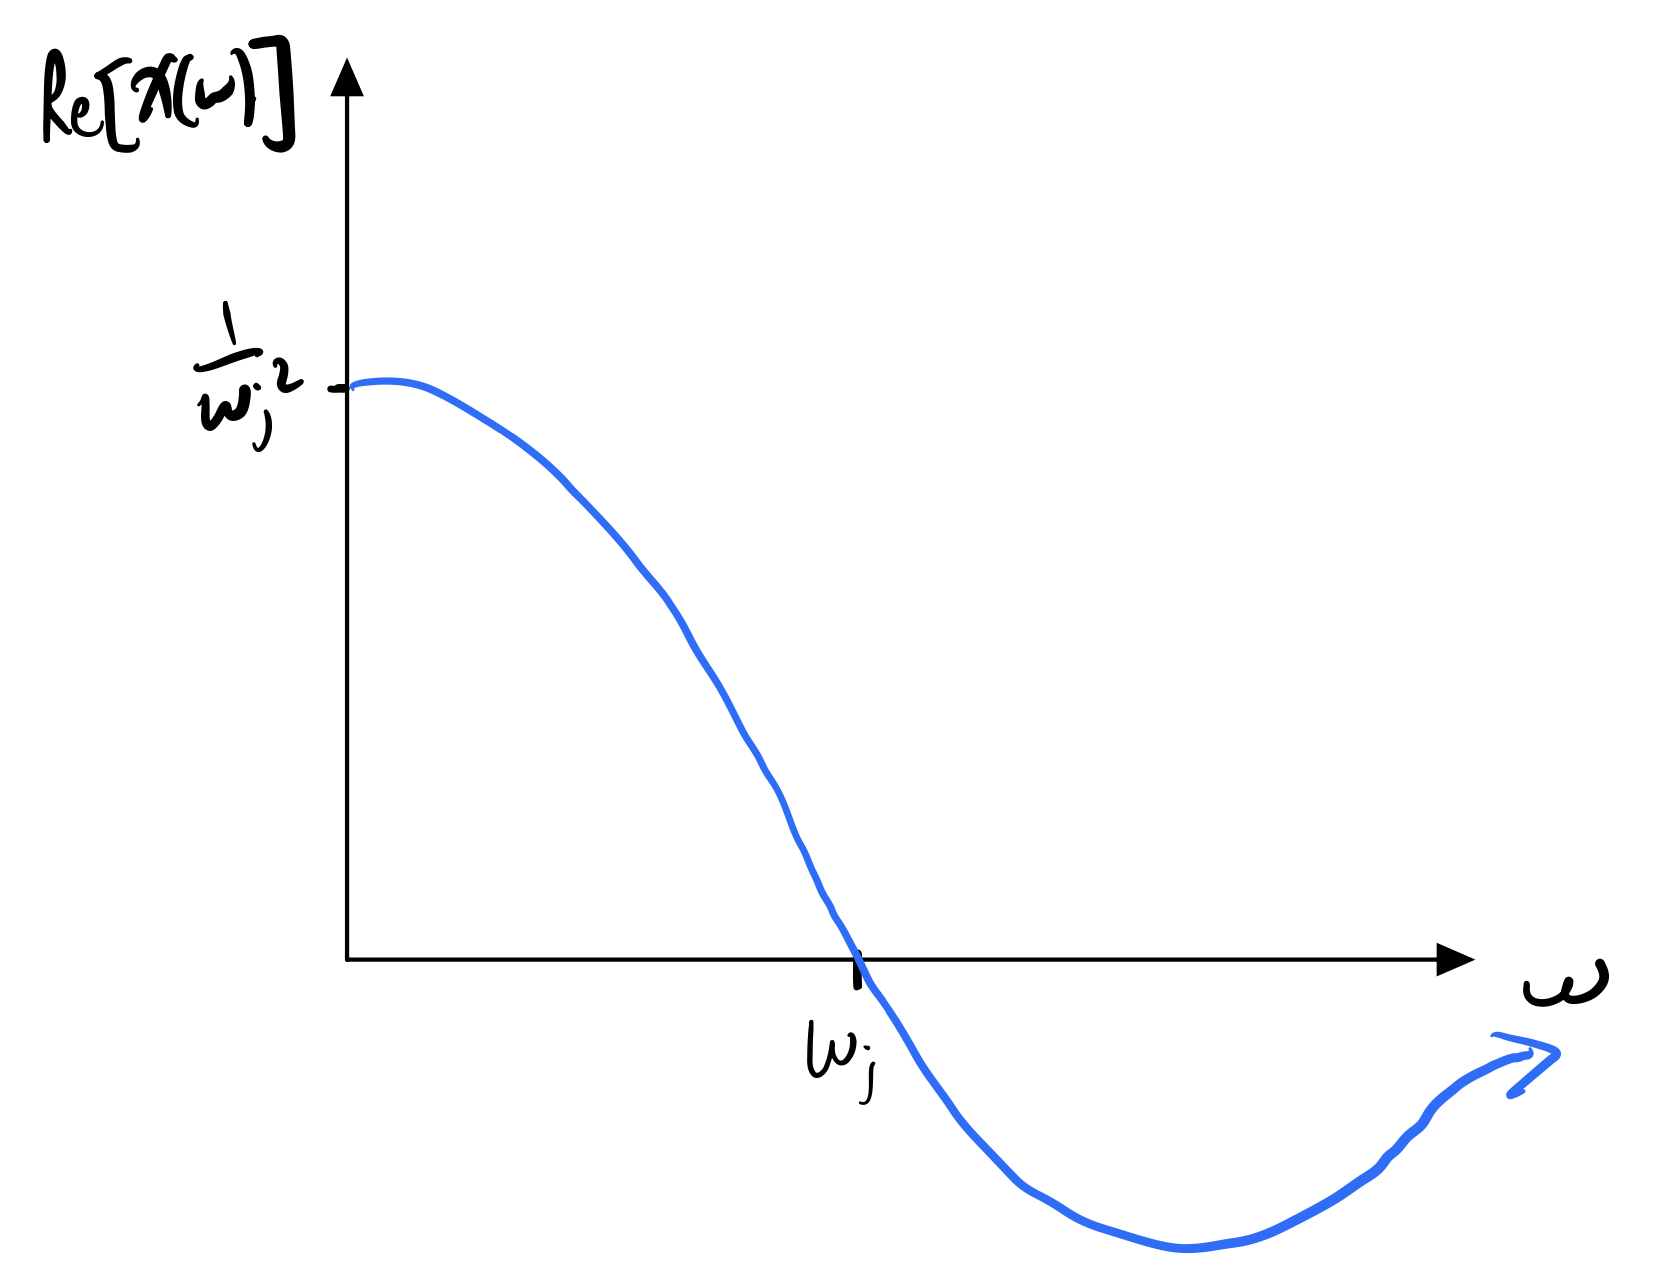
\includegraphics[scale=0.35]{Lectures/Images/lec14-rechi.png}
    \end{center}

    What is the significance of this? Recall that:
    \begin{equation}
        n(\omega) = \sqrt{\frac{\e(\omega)}{\e_0}}
    \end{equation}
    so $\dod{n}{\omega}$ is negative in some range $\omega$, corresponding to \emph{anomalous dispersion}. c.f. normal dispersion with $\dod{n}{\omega} > 0$, which occurs in water and glass. From Snell's law, we know that blue light is deflected more than red (for anomalous dispersion, the opposite holds). Note that looking at $\e(\omega)$ (specializing temporarily to $\gamma = 0$) then:
    \begin{equation}
        \e(\omega) = 1 + \frac{e^2}{\e_0m}\sum_j \frac{N_j}{\omega_j^2 - \omega^2}
    \end{equation}
    so $\e(\omega)$ also has places where it is a growing function of $\omega$ and so $\dod{n}{\omega} > 0$.
    
    Note that we can have cases where phase velocity is faster than the speed of light, and there are even cases where the group velocity is faster than the speed of light. Of course, it is impossible to transmit information faster than the speed of light - so what happens here? If $\dod{\omega}{k} > c$, then we are tuning very close to resonance, in which case we have heavy absorption.

    Question - why is normal dispersion more prevalent in nature? To answer is the Kramers-Kronig relation. Recall:
    \begin{equation}
        \Re[\chi(\omega)] = \frac{2}{\pi}\mathcal{P}\int_0^\infty d\omega'\frac{\Im[\chi(\omega')]\omega'}{\omega'^2 - \omega^2}
    \end{equation}
    If $\Im[\chi(\omega)] > 0$ we have attenuation. If we differentiate this formula w.r.t. $\omega^2$ we have:
    \begin{equation}
        \frac{\text{d}\Re[\chi(\omega)]}{\text{d}\omega^2} = \frac{2}{\pi}\mathcal{P}\int_0^\infty d\omega' \frac{\Im[\chi(\omega')]^2\omega \omega'}{(\omega'^2 - \omega^2)^2}
    \end{equation}
    so we seemed to have proven that \emph{all} material has normal dispersion - in contrast to the fact that we just showed that the Lorentz model can give rise to anomalous dispersion (and in fact real materials also show this)! Where did we go wrong? We forgot about the principal value prescription, namely we avoid the $\e$-ball around $\omega' = \omega$ and then take $\e \to 0$ at the end:
    \begin{equation}
        \int_0^\infty d\omega' = \lim_{\e \to 0}\left[\int_0^{\omega - \e}d\omega' + \int_{\omega + \e}^{\infty}d\omega'\right]
    \end{equation}
    So long as $\chi(\omega)$ is well-behaved, then this is ok. But if $\omega$ is near a resonance of $\chi$, e.g. $\omega = \omega_j$, then the something strange happens around the pole, and this is indeed what gives rise to the anomalous dispersion, though we don't have time to go into this in detail.

    Note that $\lim_{\omega \to 0} \sigma(\omega) =0$, which is the sense in which the medium is non-conducting. This is the $R \to \infty$ limit of the DC current Ohm's Law $I = frac{V}{R}$.

    \item Plasma/Conductor. In this limit we set $\omega_j = 0$, in which case:
    \begin{equation}
        \frac{\e(\omega)}{\e_0} = 1 - \frac{1}{\e_0}\frac{Ne^2/m}{\omega^2 + i\omega\gamma}
    \end{equation}
    assuming $\gamma$ is all the same. The conductivity becomes:
    \begin{equation}
        \sigma(\omega) = i\omega\frac{Ne^2/m}{\omega^2 + i\omega\gamma}
    \end{equation}
    with $N$ the number of electrons per unit volume. In the limit $\omega \ll \gamma$, we have:
    \begin{equation}
        \frac{\e(\omega)}{\e_0} = 1 + i\frac{Ne^2}{\e_0m \omega\gamma}
    \end{equation}
    and:
    \begin{equation}
        \sigma(\omega) = \frac{Ne^2}{\omega\gamma}
    \end{equation}

    in particular, DC conductivity is nonzero. This agrees with our intuition that in a plasma, if we turn on a constant electric field the charges start moving, producing a nonzero DC current $\v{J} = \sigma \v{E}$. Here you got a condensed matter class for the price of an EM class, because we've just derived the Drude model of conductivity, which is what most CM classes open with.

    The permittivity is:
    \begin{equation}
        \frac{\e(\omega)}{\e_0} = 1 + \frac{i\sigma}{\e_0 \omega} \stackrel{\omega\ll \frac{\sigma}{\e_0}}{\to} \frac{\sigma}{\e_0\omega}
    \end{equation}
    Note that $\abs{\frac{\e(\omega)}{\e_0}}$ is large in this limit, and $\e(\omega)$ is purely imaginary. What does this all mean? If we look at the index of refraction:
    \begin{equation}
        n(\omega) = \sqrt{\frac{\e(\omega)}{\e_0}} = \frac{1+i}{\sqrt{2}}\sqrt{\frac{\sigma}{\e_0\omega}}
    \end{equation}
    where we have used $i = e^{i\frac{\pi}{2}}$ so $\sqrt{i} = e^{i\frac{\pi}{4}} = \frac{1 + i}{\sqrt{2}}$.

    If we have a wave $\psi(z, t) = e^{i(kz - \omega t)}$, we have $k = \frac{\omega}{c/n}$, and in particular:
    \begin{equation}
        k = (1+i)\sqrt{\frac{\mu_0 \omega\sigma}{2}}
    \end{equation}
    so, we shine light on the metal, and the wave propagates with the $k$ above; the real part corresponds to oscillation, and the imaginary part leads to exponential decay:
    \begin{equation}
        \psi(z, t) = e^{-i\omega t}e^{i(\text{Re}(k) + i\text{Im}(k))z} = e^{-i\omega t}e^{iz/\delta}e^{-z/\delta}
    \end{equation}
    where:
    \begin{equation}
        \delta = \sqrt{\frac{2}{\mu_0\omega\sigma}}
    \end{equation}
    where $\delta$ is the skin depth, i.e. the length scale upon which the wave decays by $1/e$. What we find is that the electric field exponentially decays in the material.

    Everything we've said thus far is for $\omega \ll \gamma$. What happens in teh opposite limit of $\omega \gg \gamma$? There:
    \begin{equation}
        \frac{\e(\omega)}{\e_0} = 1 - \frac{\omega_p^2}{\omega^2}
    \end{equation}
    \begin{equation}
        \sigma(\omega) = i\frac{\e_0\omega_p^2}{\omega}
    \end{equation}
    where $\omega_p$ is the plasma frequency:
    \begin{equation}
        \omega_p^2 = \frac{Ne^2}{\e_0 m}
    \end{equation}
    The situation is the opposite as before. We have a real $\e(\omega)$ and an imaginary $\sigma(\omega)$. Recall that:
    \begin{equation}
        \avg{\hat{\v{J}}(\omega)} = \sigma(\omega)\avg{\hat{\v{E}}(\omega)}
    \end{equation}
    If $\sigma$ is imaginary, then there is a $\pi/2$ phase difference between $\v{E} \sim e^{-i\omega t}$ and $\v{J} \sim e^{i\frac{\pi}{2} - i\omega t}$. The other comment is that:
    \begin{equation}
        n(\omega) = \sqrt{\frac{\e(\omega)}{\e_0}} = \sqrt{1 - \frac{\omega_p^2}{\omega^2}}
    \end{equation}
    which is real for $\omega > \omega_p$. In this region, $n(\omega)$ is an increasing function of $\omega$ (normal dispersion). The flip side is that for $\omega < \omega_p$, then $n(\omega)$ is imaginary, and we have the penetration/decay length:
    \begin{equation}
        \delta = \frac{c}{\sqrt{\omega_p^2 - \omega^2}}
    \end{equation}
    This is physically relevant in that radio waves are reflected by the ionosphere.
\end{itemize}


